
%% bare_conf.tex
%% V1.4
%% 2012/12/27
%% by Michael Shell
%% See:
%% http://www.michaelshell.org/
%% for current contact information.
%%
%% This is a skeleton file demonstrating the use of IEEEtran.cls
%% (requires IEEEtran.cls version 1.8 or later) with an IEEE conference paper.
%%
%% Support sites:
%% http://www.michaelshell.org/tex/ieeetran/
%% http://www.ctan.org/tex-archive/macros/latex/contrib/IEEEtran/
%% and
%% http://www.ieee.org/

%%*************************************************************************
%% Legal Notice:
%% This code is offered as-is without any warranty either expressed or
%% implied; without even the implied warranty of MERCHANTABILITY or
%% FITNESS FOR A PARTICULAR PURPOSE! 
%% User assumes all risk.
%% In no event shall IEEE or any contributor to this code be liable for
%% any damages or losses, including, but not limited to, incidental,
%% consequential, or any other damages, resulting from the use or misuse
%% of any information contained here.
%%
%% All comments are the opinions of their respective authors and are not
%% necessarily endorsed by the IEEE.
%%
%% This work is distributed under the LaTeX Project Public License (LPPL)
%% ( http://www.latex-project.org/ ) version 1.3, and may be freely used,
%% distributed and modified. A copy of the LPPL, version 1.3, is included
%% in the base LaTeX documentation of all distributions of LaTeX released
%% 2003/12/01 or later.
%% Retain all contribution notices and credits.
%% ** Modified files should be clearly indicated as such, including  **
%% ** renaming them and changing author support contact information. **
%%
%% File list of work: IEEEtran.cls, IEEEtran_HOWTO.pdf, bare_adv.tex,
%%                    bare_conf.tex, bare_jrnl.tex, bare_jrnl_compsoc.tex,
%%                    bare_jrnl_transmag.tex
%%*************************************************************************

\documentclass[conference,reqno]{IEEEtran}

\usepackage{graphicx}
\graphicspath{ {images/}{images/figure1/}{images/figure2/}{images/figure3/} {images/edges/}}
%\graphicspath{{images/failures/}}
%\graphicspath{{images/figure1/}}

\usepackage{amssymb}
\usepackage{amsmath}
\usepackage{adjustbox}
\usepackage{url}
% url.sty was written by Donald Arseneau. It provides better support for
% handling and breaking URLs. url.sty is already installed on most LaTeX
% systems. The latest version and documentation can be obtained at:
% http://www.ctan.org/tex-archive/macros/latex/contrib/url/
% Basically, \url{my_url_here}.

% correct bad hyphenation here
\hyphenation{op-tical net-works semi-conduc-tor}

\begin{document}

\title{UGAN: Underwater Image Restoration using Generative Adversarial Networks}

\author{\IEEEauthorblockN{Cameron Fabbri}
\IEEEauthorblockA{Information Directorate\\
Air Force Research Laboratory \\
Rome, NY, USA.\\
cameron.fabbri@us.af.mil}
\and
\IEEEauthorblockN{Md Jahidul Islam}
\IEEEauthorblockA{University of Minnesota- Twin Cities\\
MN, USA.\\
islam034@umn.edu }
\and
\IEEEauthorblockN{Junaed Sattar}
\IEEEauthorblockA{University of Minnesota- Twin Cities\\
MN, USA.\\
junaed@umn.edu
}}

% for over three affiliations, or if they all won't fit within the width
% of the page, use this alternative format:
% 
%\author{\IEEEauthorblockN{Michael Shell\IEEEauthorrefmark{1},
%Homer Simpson\IEEEauthorrefmark{2},
%James Kirk\IEEEauthorrefmark{3}, 
%Montgomery Scott\IEEEauthorrefmark{3} and
%Eldon Tyrell\IEEEauthorrefmark{4}}
%\IEEEauthorblockA{\IEEEauthorrefmark{1}School of Electrical and Computer Engineering\\
%Georgia Institute of Technology,
%Atlanta, Georgia 30332--0250\\ Email: see http://www.michaelshell.org/contact.html}
%\IEEEauthorblockA{\IEEEauthorrefmark{2}Twentieth Century Fox, Springfield, USA\\
%Email: homer@thesimpsons.com}
%\IEEEauthorblockA{\IEEEauthorrefmark{3}Starfleet Academy, San Francisco, California 96678-2391\\
%Telephone: (800) 555--1212, Fax: (888) 555--1212}
%\IEEEauthorblockA{\IEEEauthorrefmark{4}Tyrell Inc., 123 Replicant Street, Los Angeles, California 90210--4321}}

% make the title area
\maketitle

% As a general rule, do not put math, special symbols or citations
% in the abstract
\begin{abstract}
Autonomous underwater robots often rely on visual input for decision making due to its non-intrusive and passive nature.
However, due to many factors such as light refraction, particles in the water, and color distortion, images are often times very noisy.
This paper propose a method using Generative Adversarial Networks (GANs) to denoise underwater images, and show that these 
images provide both increased accuracy for an underwater tracking algorithm, as well as a more visually appealing image.
Furthermore, we show how recently proposed methods are able to generate a dataset for the purpose of underwater image reconstruction.
\end{abstract}

\IEEEpeerreviewmaketitle

\section{Introduction}
TODO - talk about having to go back to the same location if you want to get good/bad pairs of the ``same'' image.
Vision is a commonly used sensor in autonomous underwater robots due to its non-intrusive, passive, and energy
effecient nature. The monitoring of coral reefs \cite{shkurti2012multi}, deep ocean exploration
\cite{whitcomb2000advances}, and mapping of the seabed are all tasks suitable for autonomous robots because they
provide safety by taking the risk instead of a human. Despite the advantages vision provides, many underwater
environments can be quite noisy due to light refraction and particles present in the water. Because red wavelengths are
quickly absorbed by water, images tend to have a green or blue hue to them. As you go deeper, this worsens as more
and more red wavelengths are being absorbed. This extremely non-linear distortion has many factors such as the amount
of light present (overcast vs sunny or depth), particles in the water, time of day, and the camera being used. This may
cause difficulty in tasks such as segmentation, tracking, or classification due to their indirect or direct use of
color.

As color and illumination begin to change with the depth, vision based algorithms must be very generalizable in order
to work within the depth ranges a robot may operate in. Because of the high cost and difficulty of acquiring a
variety of underwater data, as well as the high amount of noise introduced, many algorithms may perform poorly in
these different domains. Figure 1 shows the high variability that may occur in underwater environments. A step towards a
solution to this
issue is to be able to restore the images such that they appear to be above water, i.e., with colors corrected and
particles removed. By performing a many to one mapping of these domains from underwater to not underwater (what the
image would look like in the air), algorithms that have


\begin{figure}
\centering
\begin{tabular}{p{1.7cm} p{1.7cm} p{1.7cm} p{1.7cm}}
   
   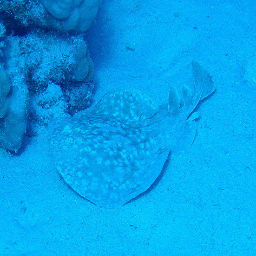
\includegraphics[width=0.8in]{n01496331_7428_f1} &
   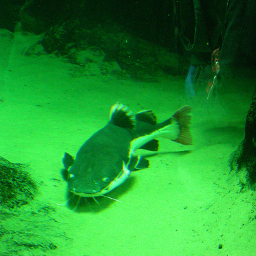
\includegraphics[width=0.8in]{n01496331_16340_f1} &
   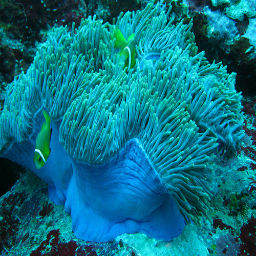
\includegraphics[width=0.8in]{n01914609_5148_f1} &
   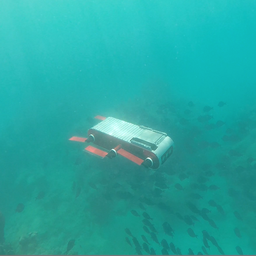
\includegraphics[width=0.8in]{robot_f1} \\
   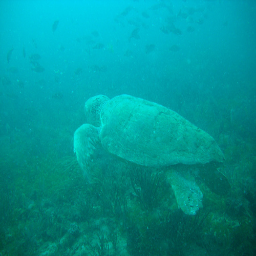
\includegraphics[width=0.8in]{n01664065_30279_f1} &
   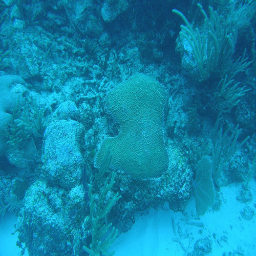
\includegraphics[width=0.8in]{n01917289_5711_f1} &
   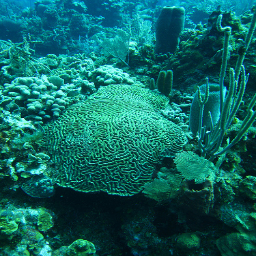
\includegraphics[width=0.8in]{n01917289_4087_f1} &
   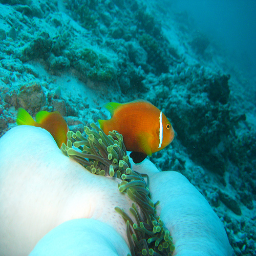
\includegraphics[width=0.8in]{n02607072_10395_f1} \\

\end{tabular}
\caption{Sample underwater images displaying the diversity of distortion that can occur. \textbf{Maybe say something about how
some images lost all color, but some kept some color for close objects.}}
\end{figure}



\noindent difficulty performing across multiple forms of noise may be able to focus only one clean domain.

Deep neural networks have been shown to be powerful non-linear function approximators, especially in the field of
vision. Often times, these networks recquire large amounts of data, either labeled or paired with ground truth.
For the problem of automatically colorizing grayscale images, paired training data is essentially free due to the
fact that any color image can be converted to black and white. However, underwater images distorted by either color
or some other visual effect lack ground truth. We use the recently proposed CycleGAN \cite{zhu2017unpaired}, which
learns to translate an image from domain $X$ to domain $Y$, as a way to generate a paired dataset. By letting $X$ be
a set of undistorted underwater images, and $Y$ be a set of distorted underwater images, we can generate an image
that appears to be underwater while retaining ground truth.

\section{Related Work}

While there have been many very successful recent approaches towards automatic colorization
\cite{zhang2016colorful,iizuka2016let}, most are focused on the task of grayscale to color.
The work of \cite{torres2005color} used an energy minimization formulation using a Markov Random Field. 
MORE RELATED BLAH. Many use physics based models to directly model the light source and such.
Most similar to our line of work is the recently proposed WaterGAN \cite{li2017watergan}, which uses
GANs for color correction of underwater images. As ground truth pairs do not exist for underwater images,
their first step is to structure a generator to create realistic underwater images. Their generator model
can be broken down into three stages: 1) Attenuation, which accounts for range-dependent attenuation of light.
2) Scattering, which models the haze effect caused by photons scattering back towards the image sensor. 3)
Vingetting, which produces a shading effect on the image corners that can be caused by certain camera lenses.
Opposed to our work, they use a GAN for generating the underwater images and Euclidean loss for color correction,
where as we use a GAN for both. Furthermore, they require depth information during the training of WaterGAN,
whereas we only require two separate image domains.

Recent work in generative models, specifically GANs, have shown great success
in areas such as inpainting \cite{pathak2016context}, style transfer \cite{Gatys_2016_CVPR}, and image-to-image
translation \cite{isola2016image,zhu2017unpaired}. This is highly due to their ability to provide a more meaningful
loss than simply the Euclidean distance, which has been shown to produce blurry results. In our work, we structure
the problem as paired image-to-image translation, using Generative Adversarial Networks (GANs) as our generative model.
Much like the work of \cite{isola2016image}, we use image pairs from two domains an input and ground truth.

\section{Method}

\subsection{Dataset Generation}
Here we describe our dataset generation process. Depth, lighting conditions, camera
model, and location are all factors that affect the amount of distortion an underwater image undergoes. Under certain
conditions, it is possible that an underwater image may have very little distortion, or none at all.
We let $I^C$ be an underwater image with no distortion, and $I^D$
be the same image with distortion. Our goal is to learn the function $f: I^D \rightarrow I^C$. Becasue of the
difficulty of collecting underwater data, more often than not only $I^D$ or $I^C$ exist, but never both.

We use the recently proposed CycleGAN \cite{zhu2017unpaired} to generate $I^D$ from $I^C$, which gives us a paired
dataset of images. Given two datasets $X$ and $Y$, where $I^C \in X$ and $I^D \in Y$, CycleGAN learns a mapping
$F: X \rightarrow Y$. Figure 2 shows paired samples generated from CycleGAN. From this paired dataset we train a
generator $G$ to learn the function $f: I^D \rightarrow I^C$. It should be noted that during our data generation process,
CycleGAN simultaneously learns a mapping $G: Y \rightarrow X$, which is similar to $f$. In section IV we show a comparison with our method.

\subsection{Adversarial Networks}
GANs \cite{goodfellow2014generative} are a class of generative models based on game theory in which a generator
network competes against an adversary. Conditioned on an image $I^D$, the generator is trained to produce an \
image to try and fool the discriminator, which is trained to distinguish be between distorted and non-distorted
underwater images. In the original GAN formulation, the goal is to solve the minimax problem: \newline

\begin{figure}
\centering
\begin{tabular}{p{1.7cm} p{1.7cm} p{1.7cm} p{1.7cm}}
   
   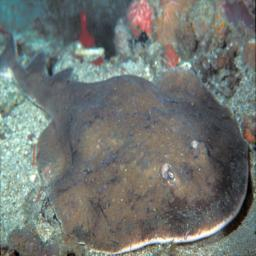
\includegraphics[width=0.8in]{n01496331_873_X} &
   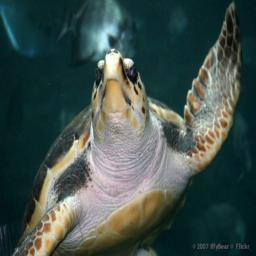
\includegraphics[width=0.8in]{n01664065_4022_X} &
   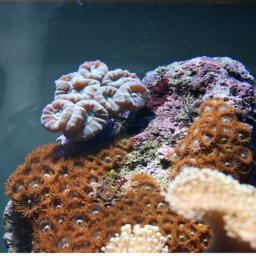
\includegraphics[width=0.8in]{n01917289_889_X} &
   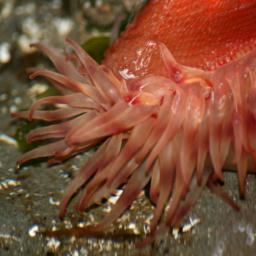
\includegraphics[width=0.8in]{n01914609_116_X} \\
   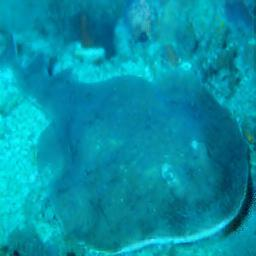
\includegraphics[width=0.8in]{n01496331_873_Y} &
   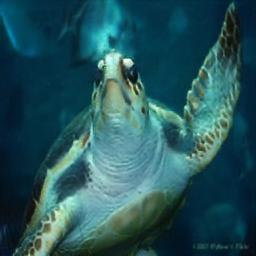
\includegraphics[width=0.8in]{n01664065_4022_Y} &
   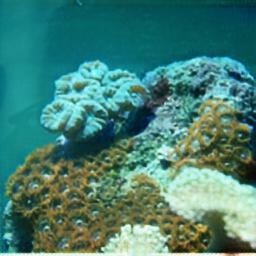
\includegraphics[width=0.8in]{n01917289_889_Y} &
   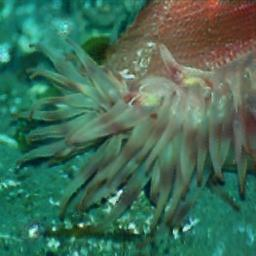
\includegraphics[width=0.8in]{n01914609_116_Y} \\

\end{tabular}
\caption{Paired samples of ground truth and distorted images generated by CycleGAN. Top row: Ground truth.
Bottom row: Generated samples.}
\end{figure}


\begin{equation}
\begin{aligned}
   \min\limits_{G}\max\limits_{D} \mathbb{E} & _{I^C \sim p_{train}(I^C)} [logD(I^C)] + \\
   \mathbb{E} & _{I^D \sim p_{gen}(I^D)}[log(1 - D(G(I^D)))]
\end{aligned}
\end{equation}

\noindent Note for simplicity in notation, we will further omit $I^C \sim p_{train}$ and $I^D \sim p_{gen}$. In this
formulation, the discriminator is hypothesized as a classifier with a sigmoid cross entropy loss function, which in
practice may lead to issues such as the vanish gradient and mode collapse. There have been many recent works which
hypothesize a different loss function for the discriminator
\cite{mao2016least,arjovsky2017wasserstein,gulrajani2017improved,zhao2016energy}. We focus on the Wasserstein GAN
(WGAN) \cite{arjovsky2017wasserstein} formulation, which proposes to use the Earth-Mover or \textit{Wasserstein-1}
distance $W$ by constructing a value function using the Kantorovich-Rubinstein duality \cite{villani2008optimal}.
In this formulation, $W$ is approximated given a set of $k$-Lipschitz functions $f$ modeled as neural networks. To
ensure $f$ is $k$-Lipschitz, the weights of the discriminator are clipped to some range $[-c, c]$. In our work, we
adopt the Wasserstein GAN with gradient penalty (WGAN-GP) \cite{gulrajani2017improved}, which instead of clipping
network weights like in \cite{arjovsky2017wasserstein}, ensures the Lipschitz constraint by enforcing a soft
constraint on the gradient norm of the discriminator's output with respect to its input. Following
\cite{gulrajani2017improved}, our new objective then becomes

\begin{equation}
\begin{aligned}
   \mathcal{L}_{WGAN}(G,D) = \mathbb{E} [D(I^C)] - \mathbb{E} & [D(G(I^D))] + \\
   \lambda_{GP} \mathbb{E} & _{\hat{x} \sim \mathbb{P}_{\hat{x}}} [(|| \nabla_{\hat{x}} D(\hat{x})||_2 -1)^2 ],
\end{aligned}
\end{equation}

%\begin{equation}
%\begin{aligned}
%   \mathcal{L}_{GAN} = \mathbb{E}_{I^D \sim p_{gen}(I^D)} [D(I^D)] - \mathbb{E} & _{I^C \sim p_{train}(I^C)} [D(I^C)] + \\
%   \lambda \mathbb{E} & _{\hat{x} \sim \mathbb{P}_{\hat{x}}} [(|| \nabla_{\hat{x}} D(\hat{x})||_2 -1)^2 ].
%\end{aligned}
%\end{equation}

\noindent where $\mathbb{P}_{\hat{x}}$ is defined as samples along straight lines between pairs of points coming from
the true data distribution and the generator distribution, and $\lambda_{GP}$ is a weighing factor. In order to give $G$
some sense of ground truth, as well as capture low level frequencies in the image, we also consider the $L1$ loss

\begin{equation}
   \mathcal{L}_{L1} = \mathbb{E} [ || I^C - G(I^D) ||_1 ].
\end{equation}
%\begin{equation}
%   \mathcal{L}_{L1} = \mathbb{E}_{I^D \sim p_{gen}, I^C \sim p_{train}} [ || I^C - G(I^D) ||_1 ].
%\end{equation}

\noindent Combining these, we get our final objective function for our network, which we call Underwater GAN (UGAN),

\begin{equation}
   \begin{aligned}
      \mathcal{L}_{UGAN}^* = \min\limits_{G}\max\limits_{D} \mathcal{L}_{WGAN}(G,D) + \lambda_{1} \mathcal{L}_{L1}(G).
   \end{aligned}
\end{equation}


\subsection{Image Gradient Difference Loss}
Often times generative models produce blurry images. We explore a strategy to sharpen these predictions by
directly penalizing the differences of image gradient predictions in the generator, as proposed by
\cite{mathieu2015deep}. Given a ground truth image $I^C$, predicted image $I^P = G(I^C)$, and $\alpha \geq 1$, the
Gradient Difference Loss (GDL) is given by

\begin{equation}
   \begin{aligned}
      \mathcal{L}_{GDL}(I^C, I^P) = \\ \sum\limits_{i,j} || & I^C_{i,j} - I^C_{i-1,j}| - | I^P_{i,j} - I^P_{i-1,j}||^{\alpha} + \\
      || & I^C_{i,j-1} - I^C_{i,j}| - | I^P_{i,j-1} - I^P_{i,j}||^{\alpha},
   \end{aligned}
\end{equation}

\noindent In our experiments, we denote our network as UGAN-P when considering the GDL, which can be expressed as

\begin{equation}
   \begin{aligned}
      \mathcal{L}_{UGAN-P}^* = \min\limits_{G}\max\limits_{D} \mathcal{L}_{WGAN}(G,D) + & \\
      \lambda_{1} \mathcal{L}_{L1}(G) + & \lambda_{2} \mathcal{L}_{GDL}
   \end{aligned}
\end{equation}


\subsection{Network Architecture and Training Details}
Our generator network is a fully convolutional encoder-decoder, similar to the work of \cite{isola2016image}, which is
designed as a ``U-Net'' \cite{ronneberger2015u} due to the structural similarity between input and output.
Encoder-decoder networks downsample (encode) the input via convolutions to a lower dimensional embedding, in which
this embedding is then upsampled (decode) via transpose convolutions to reconstruct an image. The advantage of using
a ``U-Net'' comes from explicitly preserving spatial dependencies produced by the encoder, as opposed to relying on the
embedding to contain all of the information. This is done by the addition of ``skip connections'', which concatenate
the activations produced from a convolution layer $i$ in the encoder to the input of a transpose convolution layer
$n-i+1$ in the decoder, where $n$ is the total number of layers in the network. Each convolutional layer in our
generator uses kernel size $4 \times 4$ with stride 2. Convolutions in the encoder portion of the network are followed
by batch normalization \cite{pmlr-v37-ioffe15} and a leaky ReLU activation with slope $0.02$, while transpose
convolutions in the decoder are followed by a ReLU activation \cite{nair2010rectified} (no batch norm in the decoder).
Exempt from this is the last layer of the decoder, which uses a TanH nonlinearity to match the input distribution of
$[-1, 1]$. 

Our discriminator is modeled after that of \cite{radford2015unsupervised}, except no batch normalization is used. This
is due to the fact that we penalize the norm of the discriminator's gradient with respect to each input individually,
which batch normalization would invalidate. The authors of \cite{gulrajani2017improved} recommend layer normalization
\cite{ba2016layer}, but we found no significant improvements. In particular, the use of instance normalization
\cite{ulyanov2016instance} in the generator has been shown to improve quality, but we leave that for future work.
In all of our experiments, we use $\lambda_{1} = 100$, $\lambda_{GP} = 10$, batch size of 32, and the Adam Optimizer
\cite{kingma2014adam} with learning rate $1e-4$. Following WGAN-GP, the discriminator is updated $n$ times for every
update of the generator, where $n = 5$. For UGAN-P, we set $\lambda_{2} = 1.0$. Our implementation was done using the
Tensorflow library \cite{abadi2016tensorflow}.
\footnote{Code is available at https://github.com/cameronfabbri/Underwater-Color-Correction}
All networks were trained from scratch on a GTX 1080 for 100 epochs. Inference on the GPU takes on average $ 0.0138s$,
which is about 72 Frames Per Second (FPS). On a CPU (Intel Core i7-5930K), inference takes on average $ 0.1244s$, which
is about 8 FPS. We find both of these measures acceptable for underwater tasks.

\section{Experiments}
\subsection{Datasets}
We used several subsets of Imagenet \cite{deng2009imagenet} for training and evaluation of our methods. We also
evaluate a tracking algorithm on a diving video taken from Youtube
\footnote{https://www.youtube.com/watch?v=QmRFmhILd5o}. Subsets of Imagenet containing underwater images
were selected for the training of CycleGAN, and manually separated into two classes. We let $X$ be the set of
underwater images with no distortion, and $Y$ be the set of underwater images with distortion. $X$ contained 6143
images, and $Y$ contained 1817 images. We then trained CycleGAN to learn the mapping $F: X \rightarrow Y$, such that
images from $X$ appeared to have come from $Y$. Finally, our image pairs for training data were generated by distorting
all images in $X$ with $F$. Figure 2 shows sample training pairs. When comparing with CycleGAN, we used a test set
of 56 images acquired from Flickr \footnote{How do I cite Flickr}.

\subsection{Evaluation}
We train UGAN and UGAN-P on the image pairs generated by CycleGAN, and evaluate on the images from the
test set, $Y$. Note that these images do not contain any ground truth, as they are original distorted images from
Imagenet. Images for training and testing are of size $256 \times 256 \times 3$ and normalized between $[-1, 1]$.
Figure 3 shows samples from the test set. Notably, these images contain varying amounts of noise. Both UGAN and UGAN-P
are able to recover lost color information, as well as correct any color information this is present. 

While many of the distorted images contain a blue or green hue over the entire image space, that is not always the case.
In certain environments,
it is possible that objects close to the camera are undistorted with correct colors, while the background
of the image contains distortion. In these cases, we would like the network to only correct parts of the image that
appear distorted. The last row in Figure 3 shows a sample of such an image. The orange of the clownfish is left
unchanged while the distorted sea anemone in the background has its color corrected.

We use three metrics for a quantitative evaluation. First, we compare to CycleGAN, as it inherently learns an inverse
mapping during the training of $F: X \rightarrow Y$, using the Canny edge detector
\cite{canny1986computational} as it provides a color agnostic evaluation of the images in comparison to ground truth.
Second, we compare local image patches to provide sharpness metrics on our images. Lastly, we show how an existing
tracking algorithm for an underwater robot improves performance with generated images.

\begin{figure}
\centering
\begin{tabular}{p{1.7cm} p{1.7cm} p{1.7cm}}

   ~\quad Original & ~\quad UGAN & \quad UGAN-P \\

   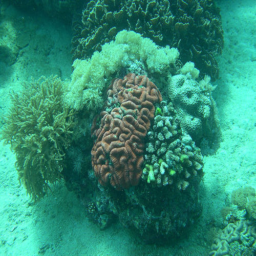
\includegraphics[width=0.8in]{n01917289_4982_real} &
   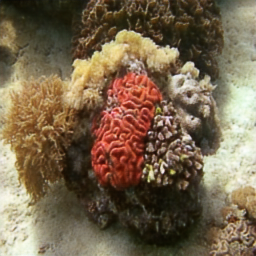
\includegraphics[width=0.8in]{n01917289_4982_gen_0} &
   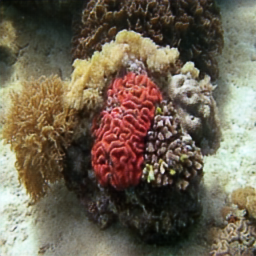
\includegraphics[width=0.8in]{n01917289_4982_gen_1} \\

   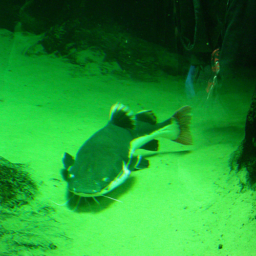
\includegraphics[width=0.8in]{n01496331_16340_real} &
   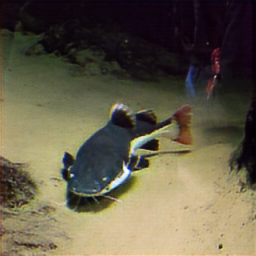
\includegraphics[width=0.8in]{n01496331_16340_gen_0} &
   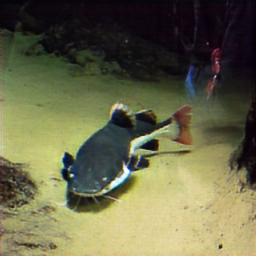
\includegraphics[width=0.8in]{n01496331_16340_gen_1} \\
   
   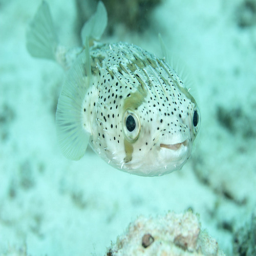
\includegraphics[width=0.8in]{n01496331_22183_real} &
   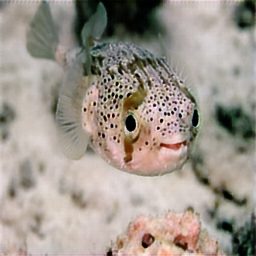
\includegraphics[width=0.8in]{n01496331_22183_gen_0} &
   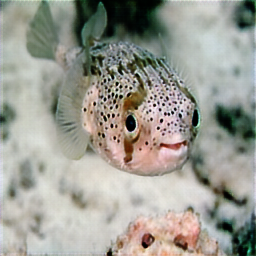
\includegraphics[width=0.8in]{n01496331_22183_gen_1} \\
   
   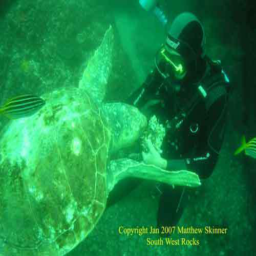
\includegraphics[width=0.8in]{n01664065_29738_real} &
   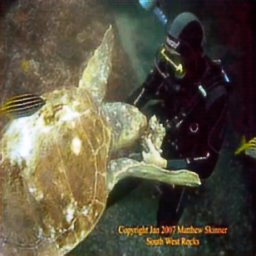
\includegraphics[width=0.8in]{n01664065_29738_gen_0} &
   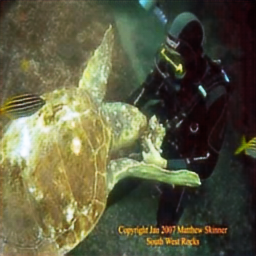
\includegraphics[width=0.8in]{n01664065_29738_gen_1} \\
   
   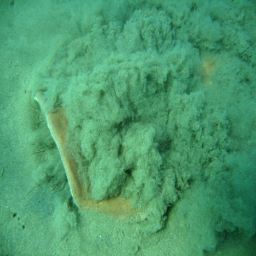
\includegraphics[width=0.8in]{n01496331_11938_real} &
   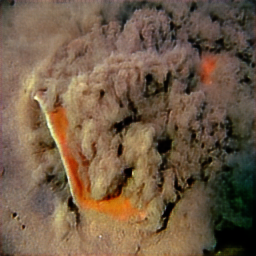
\includegraphics[width=0.8in]{n01496331_11938_gen_0} &
   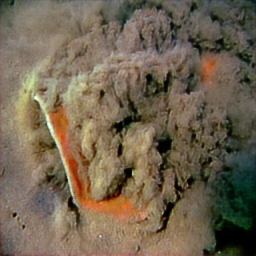
\includegraphics[width=0.8in]{n01496331_11938_gen_1} \\
   
   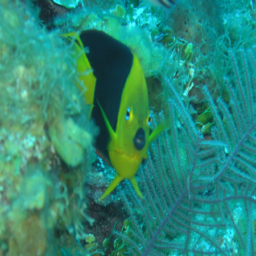
\includegraphics[width=0.8in]{n02606052_2969_real} &
   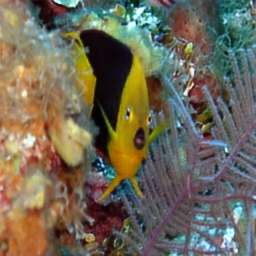
\includegraphics[width=0.8in]{n02606052_2969_gen_0} &
   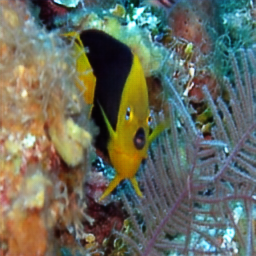
\includegraphics[width=0.8in]{n02606052_2969_gen_1} \\
   
   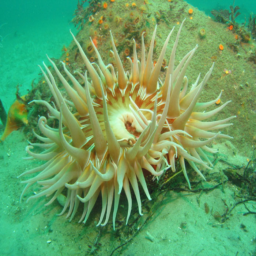
\includegraphics[width=0.8in]{n01914609_1607_real} &
   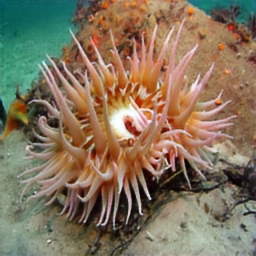
\includegraphics[width=0.8in]{n01914609_1607_gen_0} &
   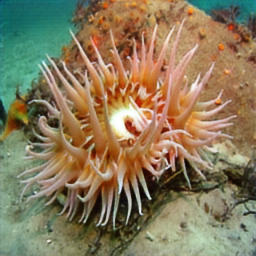
\includegraphics[width=0.8in]{n01914609_1607_gen_1} \\

   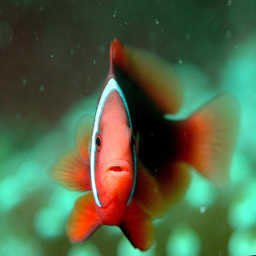
\includegraphics[width=0.8in]{n02607072_6241_real} &
   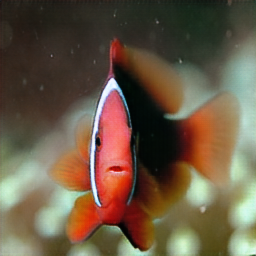
\includegraphics[width=0.8in]{n02607072_6241_gen_0} &
   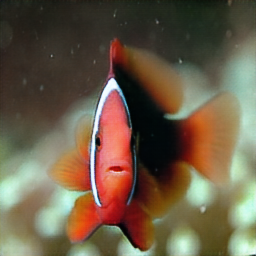
\includegraphics[width=0.8in]{n02607072_6241_gen_1} \\

\end{tabular}
\caption{Samples from our Imagenet testing set. The network can both recover color and also correct color if a small amount is present.}
\end{figure}

% Directly from the first paper on the inception score: We find that it’s important to evaluate the metric on a large
% enough number of samples (i.e. 50k) as part of this metric measures diversity.
% % Therefore we should not include it I think
% \footnote{Code for inception score can be found at https://github.com/openai/improved-gan}
%\begin{center}
%\begin{tabular}{c c c c c c}
%Samples & real & ugan & ugan-p & cyclegan \\ \hline
%Model & True Images & UGAN & UGAN-P & CycleGAN \\ \hline
%Score $\pm$ std. & $5.69 \pm 0.23$ & $6.18 \pm 0.35$ & $6.30 \pm 0.32$ & $6.37 \pm 0.43$ \\ \hline
%\end{tabular}
%\end{center}

\subsection{Comparison to CycleGAN}
It is important to note that during the process of learning a mapping $F: X \rightarrow Y$, CycleGAN also learns a
mapping $G: Y \rightarrow X$. Here we show that UGAN and UGAN-P provide superior performance. We use a Canny edge
detector \cite{canny1986computational} to provide a color agnostic evaluation of the images, as the original image
contains distorted colors. Figure 4 shows the resulting images. We noticed that CycleGAN was mostly able to restore
color, however the images contained various amounts noise. Because restoring color information should not alter the
overall structure of the image, we measure the distance in the image space between the edges found in the original 
and the generated images. Table 1 provides the measurements from Figure 4, as well as the average over the entire
dataset.

% I would like this table to match up with the figure showing edge detections. I wasn't able to
% get letters on the left side at each row though.
\begin{table}
\centering
\caption{Distances in image space}
\begin{tabular}{| c | c | c | c |}
   \hline
   Row/Method & CycleGAN & UGAN & UGAN-P \\ \hline
   A          & 116.45 & 85.71  & 86.15  \\ \hline
   B          & 114.49 & 97.92  & 101.01 \\ \hline
   C          & 120.84 & 96.53  & 97.57  \\ \hline
   D          & 129.27 & 108.90 & 110.50 \\ \hline
   Mean       & 111.60 & 94.91  & 96.51 \\ \hline
\end{tabular}
\end{table}

\newpage

\begin{figure}
\centering
\begin{tabular}{p{1.7cm} p{1.7cm} p{1.7cm} p{1.7cm}}
  
   ~\quad Original & ~CycleGAN & ~\quad UGAN & \quad UGAN-P \\

   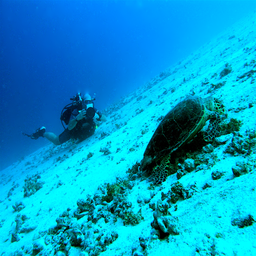
\includegraphics[width=0.8in]{1_original} &
   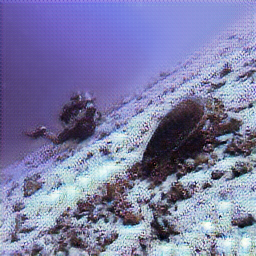
\includegraphics[width=0.8in]{1_cimg} &
   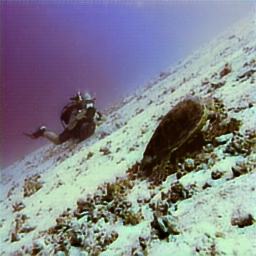
\includegraphics[width=0.8in]{1_u0img} &
   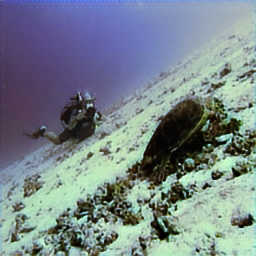
\includegraphics[width=0.8in]{1_u1img} \\ [-1ex]
   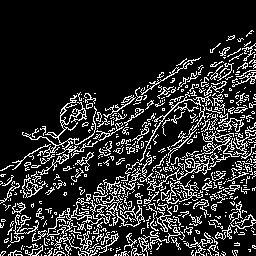
\includegraphics[width=0.8in]{1_oedges} &
   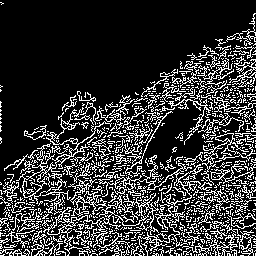
\includegraphics[width=0.8in]{1_cedges} &
   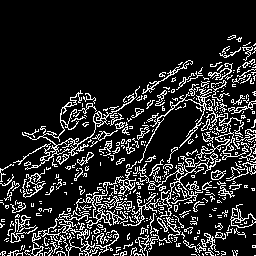
\includegraphics[width=0.8in]{1_u0edges} &
   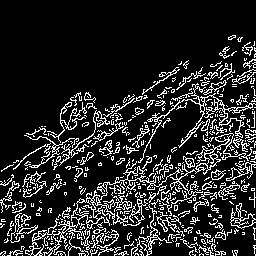
\includegraphics[width=0.8in]{1_u1edges} \\

   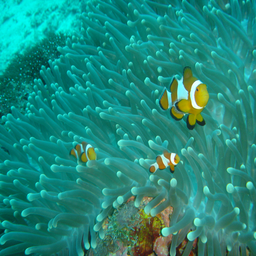
\includegraphics[width=0.8in]{2_original} &
   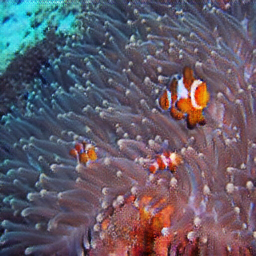
\includegraphics[width=0.8in]{2_cimg} &
   \includegraphics[width=0.8in]{2_u0img} &
   \includegraphics[width=0.8in]{2_u1img} \\ [-1ex]
   \includegraphics[width=0.8in]{2_oedges} &
   \includegraphics[width=0.8in]{2_cedges} &
   \includegraphics[width=0.8in]{2_u0edges} &
   \includegraphics[width=0.8in]{2_u1edges} \\

   \includegraphics[width=0.8in]{3_original} &
   \includegraphics[width=0.8in]{3_cimg} &
   \includegraphics[width=0.8in]{3_u0img} &
   \includegraphics[width=0.8in]{3_u1img} \\ [-1ex]
   \includegraphics[width=0.8in]{3_oedges} &
   \includegraphics[width=0.8in]{3_cedges} &
   \includegraphics[width=0.8in]{3_u0edges} &
   \includegraphics[width=0.8in]{3_u1edges} \\
   
   \includegraphics[width=0.8in]{4_original} &
   \includegraphics[width=0.8in]{4_cimg} &
   \includegraphics[width=0.8in]{4_u0img} &
   \includegraphics[width=0.8in]{4_u1img} \\ [-1ex]
   \includegraphics[width=0.8in]{4_oedges} &
   \includegraphics[width=0.8in]{4_cedges} &
   \includegraphics[width=0.8in]{4_u0edges} &
   \includegraphics[width=0.8in]{4_u1edges} \\

\end{tabular}
\caption{Running the Canny Edge Detector on sample images. Both variants of UGAN contain less noise than CycleGAN,
and are closer in the image space to the original. For each pair, the top row is the input image, and bottom row
the result of the edge detector.}
\end{figure}




% TODO definitely need help with formatting, but content is there
\begin{figure*}
\centering
\begin{tabular}{p{4.0cm} p{4.0cm} p{4.0cm} p{4.0cm}}
   
   \includegraphics[width=1.7in]{flickr_cmp} &
   \includegraphics[width=1.7in]{cgan_cmp} &
   \includegraphics[width=1.7in]{ugan_cmp} &
   \includegraphics[width=1.7in]{uganp_cmp} \\

\end{tabular}
\end{figure*}
\begin{figure*}
\begin{tabular}{p{1.9cm} p{1.9cm} p{1.9cm} p{1.9cm} p{1.9cm} p{1.9cm} p{1.9cm} p{1.9cm} }
   
   \includegraphics[width=0.8in]{flickr_crop1} &
   \includegraphics[width=0.8in]{flickr_crop2} &
   \includegraphics[width=0.8in]{cgan_crop1} &
   \includegraphics[width=0.8in]{cgan_crop2} &
   \includegraphics[width=0.8in]{ugan_crop1} &
   \includegraphics[width=0.8in]{ugan_crop2} &
   \includegraphics[width=0.8in]{ugan_crop1} &
   \includegraphics[width=0.8in]{ugan_crop2} \\

   \includegraphics[width=0.8in]{flickr_crop3} &
   \includegraphics[width=0.8in]{flickr_crop4} &
   \includegraphics[width=0.8in]{cgan_crop3} &
   \includegraphics[width=0.8in]{cgan_crop4} &
   \includegraphics[width=0.8in]{ugan_crop3} &
   \includegraphics[width=0.8in]{ugan_crop4} &
   \includegraphics[width=0.8in]{ugan_crop3} &
   \includegraphics[width=0.8in]{ugan_crop4} \\

\end{tabular}
\caption{Zooming in on comparisons.}
\end{figure*}


\subsection{Diver Tracking using Frequency-Domain Detection}
We investigate the frequency-domain characteristics of the restored images through a case-study of periodic motion tracking in sequence of images. Particularly, we compared the performance of Mixed Domain Periodic Motion (MDPM)- tracker \cite{islam2017mixed} on a sequence of images of a diver swimming in  arbitrary directions. MDPM tracker is designed for underwater robots to follow scuba divers by   tracking distinct frequency-domain signatures (high-amplitude spectra at $1$-$2$Hz) pertaining to human swimming. Amplitude spectra in frequency-domain correspond to the periodic intensity variations in image-space over time, which is often eroded in noisy underwater images \cite{shkurti2017underwater}.

Fig. \ref{mdpmStuff} illustrates the improved performance of MDPM tracker on generated images compared to the real ones. Underwater images often fail to capture the true contrast in intensity values between foreground and background due to low visibility. The generated images seem to restore these eroded intensity variations to some extent, causing much improved positive detection for MDPM tracker.

\begin{figure*}
\centering
\begin{tabular}{p{4.0cm} p{4.0cm} p{4.0cm} p{4.0cm}}
   \includegraphics[width=1.7in]{mdpm/real1} &
   \includegraphics[width=1.7in]{mdpm/real2} &
   \includegraphics[width=1.7in]{mdpm/real3} &
   \includegraphics[width=1.7in]{mdpm/real4} \\
   \includegraphics[width=1.7in]{mdpm/gen1} &
   \includegraphics[width=1.7in]{mdpm/gen2} &
   \includegraphics[width=1.7in]{mdpm/gen3} &
   \includegraphics[width=1.7in]{mdpm/gen4} \\
\end{tabular}
\vspace{4mm}

\begin{tabular}{l|c|c|c|r|}
 \cline{2-5}
 &  Correct detection & Wrong detection & Missed detection & Total \# of frames\\ \hline  \cline{2-4}
On real images  &  42 & 14 & 444 & 500  \\ \hline
On generated images  &  147 & 24 & 329 & 500  \\ \hline
\end{tabular}

\caption{Performance of MDPM tracker \cite{islam2017mixed} on both real (top row) and generated (second row) images; the Table compares the detection performance for both sets of images over a sequence of $500$ frames.   }
\label{mdpmStuff}
\end{figure*}


%Flippers of a human diver typically oscillate at frequencies between $1$ and $2$ Hz, which produces periodic intensity variations in the image-space over time. These variations correspond to distinct signatures in the frequency-domain (high-amplitude spectra at $1$-$2$Hz), which can be used for reliable detection.



\section{Conclusion}

Future work: Getting a better and larger dataset. I think that would help a great deal. Also data augmentation
after CycleGAN, such as gaussian blurring, noise, particle effect, more lighting effects etc.

\section*{Acknowledgment}

\bibliography{cambibs}
\bibliographystyle{ieeetr}

\end{document}


